\documentclass{article}
\usepackage{graphicx}
\usepackage{caption}
\usepackage{lipsum}
\usepackage{amsmath}
\usepackage{adjustbox}

\usepackage[
backend=biber,
style=apa,
]{biblatex}
\addbibresource{reference.bib}



\graphicspath{ {./images/} }

\title{MSc Dissertation Report - "Hyper-automating Enterprise Architecture (EA) by Integrating SAP Graph Metadata and Essential Project"}
\author{c1048663}
\date{August 2023}

\begin{document}
\maketitle
\section*{Acknowledge}
I would like to express my heartfelt gratitude to Sheffield Hallam University for providing me with the opportunity to pursue my research and complete this dissertation. The university's support, resources, and academic environment have been instrumental in shaping my academic journey and enabling me to achieve my goals.
Moreover, I am deeply thankful to my supervisor, Dr. Simon, for his unwavering guidance, invaluable insights, and continuous encouragement throughout this research. His expertise in the field of SAP Enterprise Architecture and his commitment to academic excellence have been instrumental in shaping the direction of this dissertation. I am grateful for his patience and dedication in providing constructive feedback, which has significantly enhanced the quality of my work.
Dr. Simon's mentorship has been transformative, and I am truly fortunate to have had the opportunity to work under his guidance. His passion for research and commitment to fostering a stimulating learning environment has inspired me to push the boundaries of my knowledge and skills.
I extend my heartfelt appreciation to Dr. Simon for his mentorship, support, and encouragement, which have been pivotal in the successful completion of this research dissertation.

\newpage
\maketitle
\section*{Abstract}
The SAP Business Technology Platform serves as a robust foundation for businesses, offering the necessary tools to build, integrate, extend, and operate applications and services seamlessly. Complementing this, Essential Architecture equips enterprises with powerful tools for designing, structuring, organizing, and managing intricate enterprise architectures, encompassing technology, processes, data, and personnel.

This dissertation explores the feasibility and advantages of automating Essential Architecture (EA) by harnessing the capabilities of SAP Graph Metadata entities and leveraging the SAP Graph and Essential Architecture APIs. The primary challenge in integrating SAP Graph with Essential Architecture stems from managing a substantial number of entities, reaching approximately 2000, including custom entities. Manual handling of this vast amount of data can result in errors and duplicate entries. Nevertheless, this challenge is effectively addressed by harnessing the APIs provided by both platforms, unlocking the potential for automating the entire process. Automating Essential Architecture through integrating SAP Graph metadata with the essential architecture presents its share of challenges, notably due to the sheer size of the SAP Graph metadata. To overcome this obstacle and ensure data accuracy, data mining algorithms prove indispensable. Utilizing association mining rules facilitates the extraction of pertinent information from the extensive SAP Graph metadata before merging it with the Essential Architecture, ensuring a streamlined and error-free integration. Crucially, the SAP Graph API furnishes metadata that details the relationships among entities. Additionally, the utilization of Linked Enterprise Data proves instrumental in organizing and connecting data seamlessly, offering efficient queries to access and retrieve linked information.

The core focus of this dissertation centers on the realization of automating essential architecture (EA) by integrating SAP Graph Metadata. The research delves into the intricacies and potentials of this integration approach, shedding light on its transformative impact in streamlining and optimizing essential project processes. The outcomes and insights drawn from this study contribute significantly to the field of enterprise architecture. The findings serve as a stepping stone for further research and real-world implementation, promising innovative and efficient solutions to tackle complex enterprise architecture challenges. As organizations continue to seek ways to enhance their operations and drive innovation, the exploration of automated Essential Architecture becomes increasingly relevant and effective.

\newpage
\tableofcontents

\newpage
\maketitle
\section{Introduction}
In today’s world business is rapidly evolving, and organizations face the pressing need to leverage advanced technologies and efficient architectures to remain competitive and innovative. The SAP Business Technology Platform stands as a testament to the transformative potential of modern enterprise solutions, empowering businesses to build, integrate, extend, and operate applications and services seamlessly. Concurrently, Essential Architecture provides indispensable tools to design, structure, organize, and manage complex essential architectures, encompassing technology, processes, data, and people. An enterprise endeavors to streamline its processes and maximize operational efficiency, and the automation of the Essential Architecture (EA) emerges as a compelling solution.

This dissertation aims to explore the feasibility and advantages of automating Essential Architecture by harnessing the capabilities of SAP Graph Metadata entities and leveraging the SAP Graph and Essential Architecture (EA) APIs. As organizations increasingly embrace digital technology, integrating SAP Graph metadata with essential architecture holds immense promise in optimizing essential project processes. However, such integration does not come without challenges.

One of the primary hurdles in the SAP Graph with Essential Architecture lies in managing the extensive numbers of entities, which can reach a staggering count of around 2000, inclusive of custom entities. The manual analysis and capture of this vast amount of data poses a significant risk of errors, duplication, and inaccuracies. Nevertheless, the adoption of the APIs provided by both platforms proves to be the key to unlocking the full potential of automation.

Automating Essential Architecture through the integration of SAP Graph metadata with the essential architecture not only streamlines processes but also enhances the quality and accuracy of data. To ensure seamless integration, data mining algorithms come to the forefront, offering valuable assistance in extracting essential information from the extensive SAP Graph metadata. The utilization of association mining rules emerges as a pivotal technique to filter pertinent data before its amalgamation with the Essential Architecture. Furthermore, the SAP Graph API proves to be an invaluable asset, providing metadata that elucidate the relationships among entities, enabling a deeper understanding of data connections. The use of Linked Enterprise Data further enriches the integration process, facilitating the seamless organization and connection of data. This, in turn, empowers users with efficient queries to access and retrieve linked information with ease.

As we delve into the heart of "Automating Essential Architecture (EA) by Integrating SAP Graph Metadata and Essential Project," this dissertation presents a comprehensive exploration of the intricacies and potentials of this integration approach. By overcoming challenges in handling vast datasets and harnessing the power of data mining techniques, this automated integration approach serves as a robust and scalable solution for enterprises seeking to optimize their architecture integration and management processes.

The findings and insights of this study hold great promise for the field of enterprise architecture, offering valuable contributions and paving the way for further research and real-world implementation. As organizations strive to navigate the complexities of the digital era, the exploration of automated Essential Architecture takes center stage, providing a pathway to enhanced efficiency and innovation.

\maketitle
\subsection{Previous Works}
While working with the SAP Graph and Essential Architecture, it is essential to delve into existing research on the SAP Graph. One such paper authored by Hwang in 2018 proposes a novel approach of implementing graph operations directly into the database engine and exposing APIs to interact with graph data. The focus of this research lies specifically on the SAP HANA database. The study involves converting SAP HANA data into a graph structure, comprising Attributes, Vertices, and Edges. Consequently, the research proceeds to develop APIs around this graph representation, simplifying the complexities of the SAP Graph by abstracting the data management layer and enhancing query performance. \parencite{hwang2018}

In addition to graph implementation, Database Reverse Engineering based on Association Rule Mining is also suggested to analyze legacy databases with inadequate documentation. This approach proves valuable in discovering conceptual schema within these databases. Notably, Pannurat's paper from 2010 \parencite{pannurat2010} explores the recreation of databases to the third form of normalization using association rule mining.

These research findings shed light on the potential of integrating SAP Graph Metadata and Essential Architecture through APIs. By building upon existing approaches, such integration promises streamlined data management, improved performance, and enhanced insights for enterprises. However, while the groundwork has been laid, further exploration and validation in real-world scenarios are crucial to fully realize the benefits of this integration for complex enterprise architecture management.

\maketitle
\subsection{The Motivation}
In today's digital era, businesses operate in a highly interconnected and data-driven environment, where the effective management and utilization of technology play a pivotal role in achieving success and competitive advantage. Among the array of technology solutions available, the SAP Business Technology Platform stands as a powerful enabler, offering a comprehensive suite of tools to build, integrate, extend, and operate applications and services. Alongside this, other cloud platforms, such as Essential Architecture and various industry-specific solutions, present valuable opportunities to enhance operational efficiency, optimize data management, and drive innovation.

The motivation behind this research dissertation lies in recognizing the ever-increasing need for seamless automation and integration of SAP with other useful cloud platforms, particularly Essential Architecture. While the SAP Business Technology Platform serves as a robust foundation for businesses, providing extensive capabilities to support their operations, it is often imperative for enterprises to leverage additional cloud platforms to cater to their specific needs and industry requirements.

\textbf{Holistic Data Connectivity –} The integration of SAP Graph with Essential Architecture and Linked Enterprise Data enables a holistic view of organization data by connecting disparate data sources. This interconnectedness fosters a comprehensive understanding of business operations and customer interactions, facilitating well-informed decision-making.

\textbf{Data Harmonization and Standardization –} Automation and integration ensure the harmonization and standardization of data across platforms, promoting consistency and accuracy. This unified approach to data management streamlines processing and reduces data redundancy.

\textbf{Enhanced Data Analysis and Insights –} The combination of SAP, Essential Architecture, and Linked Data Enterprise enriches data analytics capabilities, enabling enterprises to derive deeper insights and identify trends that drive business growth and operational efficiency.

\textbf{Research Gap –} As mentioned in previous work, the SAP Graph was used to create scalable and improved querying by creating an abstract layer. However, what remains unexplored is the automation and integration of SAP Graph to extract useful information for optimizing business processes. The existing literature lacks a comprehensive investigation into harnessing the full potential of SAP Graph by seamlessly integrating it with other platforms to derive valuable insights and support data-driven decision-making.

\maketitle
\subsection{Objective and Scope}
The primary objective of this dissertation is to provide a tool or technique to automate the SAP graph data with essential architecture. With the help of linked enterprise data to enhance data management, optimize business processes, and foster data-driven decision-making. We aim to investigate the existing literature and research on SAP Graph, Essential Architecture, and Linked Enterprise Data, to identify the potential benefits and challenges of automating and integrating these platforms. By combining SAP Graph and Essential Architecture, we seek to automate processes and utilize the data management and information layers for effective data visualization. 

In this dissertation, our primary objective is to implement Linked Enterprise Data on the SAP Graph, creating unified and easy access to SAP Graph entities' data with valuable information about the queried data. To achieve this, we will leverage the SAP Graph API to download and process metadata, utilizing the outcomes in Essential Architecture API to generate meaningful results. Furthermore, our objective includes employing machine learning techniques to extract pertinent information and simplify the entities' results, contributing to the definition of the data management and information layer within Essential Architecture.

Ultimately, our dissertation aims to demonstrate the advantages of using automation for SAP Graph and Essential Architecture, showcasing how this integration can revolutionize data management, streamline processes, and empower data-driven decision-making for enterprises.

By addressing these objectives, we intend to make a significant contribution to the field of enterprise architecture and data management, providing valuable insights and practical applications for leveraging the potential of SAP Graph and Essential Architecture through automation and integration.

\maketitle
\section{Research Design}
The Research Onion is a research methodology first proposed by Saunders in 2007 \parencite{sahay2016}. It serves as a conceptual model, with each layer resembling the layers of an onion. Starting from broad philosophical assumptions at the outer layer, the research process gradually narrows down to specific data collection and analysis at the core.

Choosing a research methodology is a critical aspect of any research project. For this dissertation, we have opted to use the Research Onion because it offers a systematic approach, guiding us through each layer in a step-by-step manner to design a well-structured and comprehensive study. Let's now delve into how the Research Onion is applied to our research.

\begin{figure}[ht!]
    \centering
    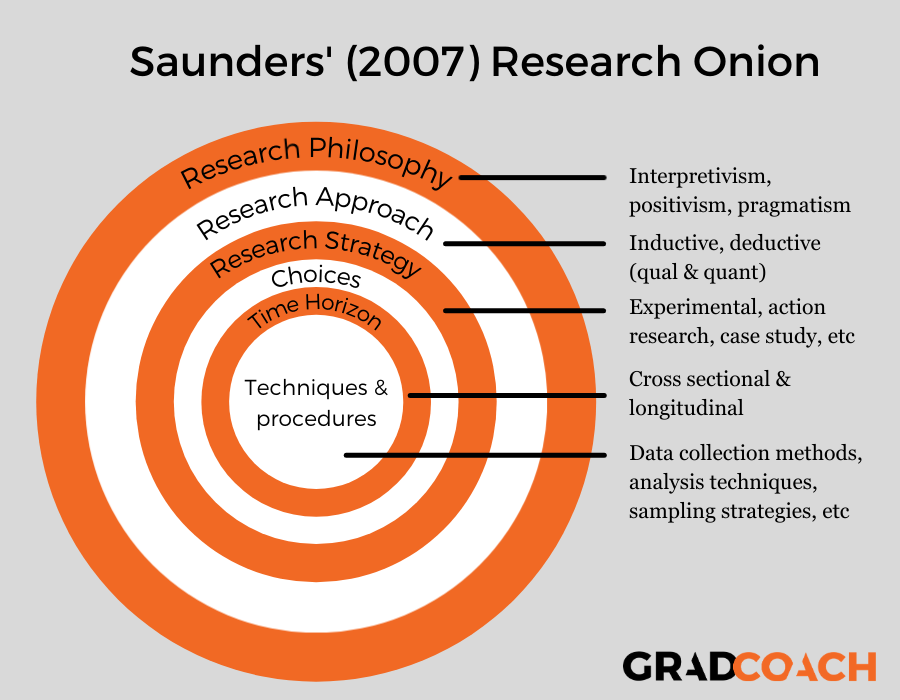
\includegraphics[scale=0.4]{onion-research}
    \caption{Saunder's 2007 Research Onion - The proposed research onion model has layers just like an onion, peeling through each layer and narrowing down to concentrate on the specific problem. \parencite{gradcoach}}
    \label{fig: onion research}
\end{figure}

\maketitle
\subsection{Philosophical Assumptions}
In research onion, the research philosophy can be either ontological or epistemological. \parencite{alababneh2020}. Ontology is the study of “what” and “how” while epistemology is the study of “how”. There are three types of research philosophy Positivism, Interpretivism, and Pragmatism. These operate on top of ontological and epistemological assumptions. In Positivism, researchers cannot include opinions because the positivist research methodology is based on objective and reality, and it is based on measurement and observations. \parencite{goldkuhl2012}. While essential architecture is based on subjectivity, positivism does not fit well with this dissertation research. Based on the other research philosophy, pragmatism provides approaches based on a practical point of view and it also lets researchers provide their point of view. Unlike positivism, pragmatism is subjective therefore pragmatism philosophy fits this dissertation.

\maketitle
\subsection{Research Approach and Strategy}
A qualitative research approach focuses on understanding and interpreting the meanings, experiences, and perceptions of individuals or groups in a specific context. It allows us to explore the complexities and nuances of the integration process, decision-making, and user experience related to the automation of SAP with Essential Architecture and Linked Enterprise Data \parencite{hammarberg2016}.

In the qualitative approach for the dissertation on SAP Graph and Essential Architecture, we evaluated the need to explore the required REST API provided by SAP Graph to determine if they are sufficient for fetching the required data. Additionally, we thoroughly examined the Essential Architecture API documentation to ensure that it supports data capture operations for data management analysis, information layer creation, and any other required functionalities.

Furthermore, the qualitative approach allows us to assess how the implementation of Linked Enterprise Data can benefit the organization. We aim to explore how data mining techniques applied to graph data can extract useful information to enhance decision-making processes.

\textbf{Rationale for Cast Study Approach -}
The rationale for adopting a case study approach in the research on "Automation and Integration of SAP with Essential Architecture" is rooted in its suitability for exploring complex, real-world integration scenarios. The case study approach allows for an in-depth examination of multiple organizations, providing a holistic understanding of the integration process. By conducting case studies in diverse organizational contexts, we gain valuable insights into how automation and integration are implemented in practice. Each organization represents a unique context with specific business processes and data structures.

The findings from these case studies can offer practical implications and actionable recommendations for organizations seeking to automate and integrate SAP with essential architecture. This broader view allows us to identify common themes, patterns, and challenges across organizations, leading to a comprehensive understanding of the research topic.

To summarize, the qualitative approach and case study strategy are well-suited for the dissertation, as they align intending to understand the experiences and decision-making processes related to the automation and integration of SAP and Essential Architecture. This approach will provide valuable insights into the complexities of integration and help identify critical factors for successful implementation. By delving into the perspectives and experiences of stakeholders and users, we can gain a deeper understanding of the challenges and opportunities presented by the automation and integration of these systems.

\maketitle
\subsection{Techniques and Procedures}
The data collection techniques employed include in-depth interviews, focus group discussions, observations, and document analysis. Participants from various organizations, including key stakeholders, IT managers, business analysts, and end-users, were interviewed to gain valuable insights into their experiences, decision-making processes, and perspectives regarding the integration process.

To gather data, SAP graph API was used to fetch the data, the data contains the entities' metadata, which is used throughout this dissertation. To store data related to the purpose of Linked Enterprise Data, the Neo4j database was utilized, allowing for efficient and effective data management and organization. Additionally, the research made use of REST APIs to extract relevant information from the SAP Graph and Essential Architecture, enabling seamless data capture operations for analysis and visualization.

For the user interface, the Python Django framework was employed, facilitating an intuitive and user-friendly platform for interaction with the integrated data. This allowed for a comprehensive view of the automation and integration process, enhancing the ability to identify challenges and opportunities presented by the integration.

Throughout the data collection process, meticulous transcription and data cleaning were conducted, ensuring the accuracy and confidentiality of participants' responses. The data was then subjected to thematic analysis, allowing for the identification of recurring patterns and themes related to the automation and integration of SAP with Essential Architecture and Linked Enterprise Data.

\begin{figure}[ht!]
    \centering
    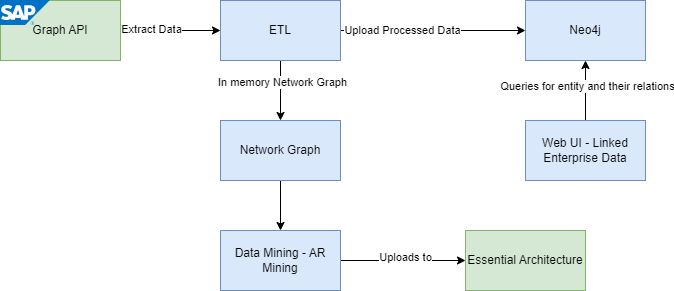
\includegraphics[width=0.75\textwidth]{techique-overview}
    \caption{SAP Graph with Essential Architecture
The flow diagram shows the integration of SAP Graph with the Essential Architecture. It shows the processes between the integration.}
    \label{fig: technique overview}
\end{figure}

In this research, the purposed Linked Enterprise Data framework was used, the data collection process involves several steps to gather and integrate information from various sources. The first step is to fetch data from the SAP Graph, which serves as a primary data source. Once the data is extracted, it undergoes an Extract, Transform, Load (ETL) process to create a network graph, which is then stored in memory. The data needs to be available for query and access purposes, producing new information, and then performing analysis and visualization as per Linked Enterprise Data were consumed. Simultaneously, another set of processed data is passed to the Neo4j graph database, where Linked Enterprise Data is organized and managed. This step ensures that the data is efficiently structured for easy access and retrieval.

To enable easy querying of the integrated data, a web-based interface is developed. This interface provides users with a user-friendly platform to access and interact with the interconnected data from SAP Graph and Linked Enterprise Data. The final step involves data mining techniques to extract relevant and useful information from the processed data. These valuable insights are then uploaded to Essential Architecture using the REST API, enriching the architecture's data management and decision-making capabilities.

By following this comprehensive data collection process, the research aims to gain a deeper understanding of the automation and integration of SAP with Essential Architecture and Linked Enterprise Data. This approach allows for a holistic view of the interconnected data, facilitating more informed decision-making processes and practical implications for real-world implementations.


\maketitle
\section{ERP and SAP Graph}
ERP is simple could base software with proper remote and web base access. ERP is the abbreviation of “Enterprise resource planning” software. Without ERP software no company can survive because it helps the companies to streamline their business processes with resource planning like how much inventory has been sold and how much it was purchased. In short, it integrates all the business processes which are necessary to run a company. Moreover, it makes communication more flexible between the different departments. Generally, the backbone of any ERP system covers five fundamental planning and managing packages finance management, human resource management, logistics., manufacturing/production, and supply chain. In the ERP solution, the first data is collected from all departments of a company. which is then hosted onto a server then it is accessible for generating reports so that accuracy and production can be improved. \parencite{anderson2023}

SAP, or “System Application and Products in Data Processing”, is a German multinational software corporation that develops enterprise software solutions. The company was founded in 1972 and is headquartered in Germany \parencite{lombardi2023}. SAP is used to rationalize business processes and resource planning. Firstly, it was System Analysis Program Development then later it was abbreviated as SAP and up to now. SAP components include ERP for core business functions, CRM for customer relationships, SCM for supply chain management, and PLM for product lifecycle. Other components cover areas such as HR, business intelligence, warehouse management, and governance. SAP S/4HANA is the next-generation ERP suite. \parencite{lombardi2023}. Originally, SAP R/1, R./2, R/3, and SAP ECC (Essential Central component) were launched as a global standard ERP solution in the world. However, the latest ERP is SAP S/4 HANA. 

SAP HANA is an in-memory database platform that combines a database management system with advanced analytics capabilities. It allows for the rapid processing of large volumes of data in real-time, enabling businesses to perform complex data analysis, gain valuable insights, and make informed decisions faster \parencite{lombardi2023}. SAP HANA also provides the foundation for SAP's next-generation ERP suite, SAP S/4HANA, offering improved performance, scalability, and agility for businesses.

Nowadays the latest debate is about SAP Cloud Essential. Sap S/4 HANA Cloud Essential is the advanced version of SAP S/4 HANA. SAP Essential is simply a cloud version to automate the business process and improve customer performance using AI Chatbots. SAP essentially helps people to understand business models. It helps people to capture data without understanding the business model. It enables us to analyze for decision-making. Moreover, customers can share both the database and the codebase of a S/4HANA instance \parencite{singh2023life}. 

Every system wants Integration. SAP Graph API is a unified API for SAP developers. It helps the developers to manage and scale up the business processes. SAP Business Technology Platform (SAP BTP) is an integrated platform provided by SAP that offers a set of services and tools to build, extend, and integrate SAP applications and solutions. It provides a flexible and scalable foundation for developing and running enterprise applications, enabling businesses to leverage the latest technologies and innovations. SAP BTP provides a unified and integrated environment for businesses to develop, integrate, and manage their applications and technologies. It supports both cloud-based and on-premises deployments, allowing organizations to choose the deployment model that best suits their needs. With SAP BTP, businesses can accelerate digital transformation, drive innovation, and gain a competitive edge in the rapidly evolving business landscape. \parencite{cox2020saps}

\maketitle
\subsection{Data Collection from SAP Graph API}
SAP Graph API (Application Programming Interface) is a unified and standardized way to access data from various SAP applications and services and enables a holistic view of the interconnectedness of business objects and processes. Developers can query the data, retrieve data, perform operations like filtering data, and explore data by analyzing connections between different entities, such as customers, products, orders, suppliers, and more. By utilizing SAP Graph, developers can build applications, services, and integrations that leverage the rich data relationships within SAP systems. It enables a more comprehensive understanding of data interdependencies, facilitates advanced analytics, and promotes agile and intelligent business operations. Moreover, it enables developers to access and interact with the data stored in SAP systems. It leverages the power of graph technology to represent and navigate relationships between entities in the SAP ecosystem.

It's important to note that SAP Graph is a relatively new technology and was introduced to provide a unified and consistent approach to accessing data across different SAP solutions. As a result, specific details and functionalities of SAP Graph may evolve as SAP continues to enhance and expand its capabilities. To interact with SAP Graph API and fetch the SAP entities metadata, below is the sequence diagram which demonstrates the interaction between the client and the SAP Graph API.

\begin{figure}[ht!]
    \centering
    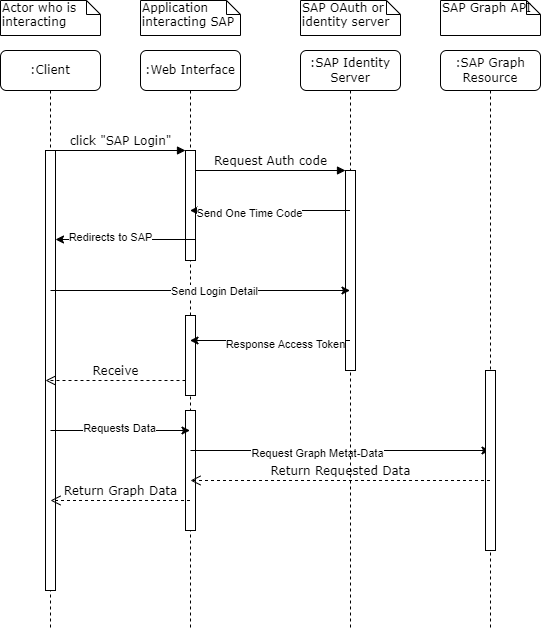
\includegraphics[scale=0.5]{sap-graph-api-interaction}
    \caption{SAP Graph API Interaction - The diagram shows the client when clicking login with the SAP button, redirects to the SAP web page, and once logged in, the client can request through a developed web application to fetch SAP Graph data.}
    \label{fig:graph-api}
\end{figure}

The SAP Graph API uses OAuth 2.0 mechanism to authorize users to access the resource. In OAuth 2.0, a web developer provides a redirect URI. This redirect URI is usually the logging-in website. Once the user clicks on Login with SAP button, the user is redirected to the SAP portal page to log in, once the user is logged in, the access token and refresh token are sent to the redirect URI. An access token is a digitally signed token called JSON Web Token or JWT, it contains scope and roles for the signing user. A refresh token is used to fetch a new access token once the user session expired.

To interact with SAP Graph API, the first need is to generate a client id and client secret from the SAP BTP portal. SAP Graph should register graph id, this is the path parameter in the SAP Graph API, in this path parameter SAP Graph fetches the list of entities metadata. There are two URLs provided by the SAP Graph API, one is for the identity server. The purpose of the identity server is to authenticate and authorize users to access the SAP resources, the second URL is the resource server URL. Lastly, the user also needs the application interface key, which will be generated by the SAP Graph API. The application interface key is passed in the HTTP Header along with the Authorization token to fetch the entities' metadata. 

\maketitle
\subsection{Web Application and SAP Data Collection}

For the dissertation, first data collection is required. The figures show the developed application for this dissertation screenshots, the screenshots showed in Figure 1 4  that user clicked the “Login with SAP” button, which opens the SAP login page. Once the user enters the correct credentials, the user is redirected to the web application, where the user can see buttons called “Sync All Entities”, “Sync with Neo4j”, and “Load Graph Network”.

\begin{figure}[ht!]
    \centering
    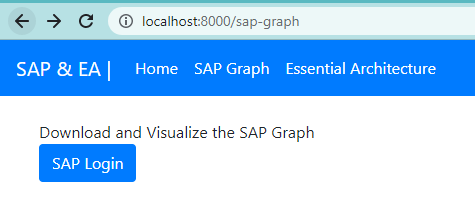
\includegraphics[scale=0.8]{sap-log-w}
    \caption{Login SAP - 
Opens an SAP Login Page for a user to enter the valid credentials
}
    \label{fig:sap-login}
\end{figure}

\begin{figure}[ht!]
    \centering
    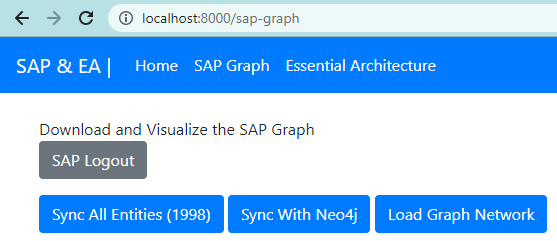
\includegraphics[scale=0.8]{sap-logged-w}
    \caption{Logged in SAP - When a user is logged in with SAP
}
    \label{fig:sap-logged-in}
\end{figure}


After the user is logged into the web application and clicked on the “Load Graph Network” it will load all the entities with their relationship with other entities. Figure 6 shows the output of the button clicked. In the figure, “sap.c4c” is represented in red color and dot symbol, “sap.s4” is represented in dark blue color and star symbol, “sap. graph” is represented in green color and triangle symbol, and “sap. hcm” is represented in purple color and diamond symbol.

\begin{figure}[ht!]
    \centering
    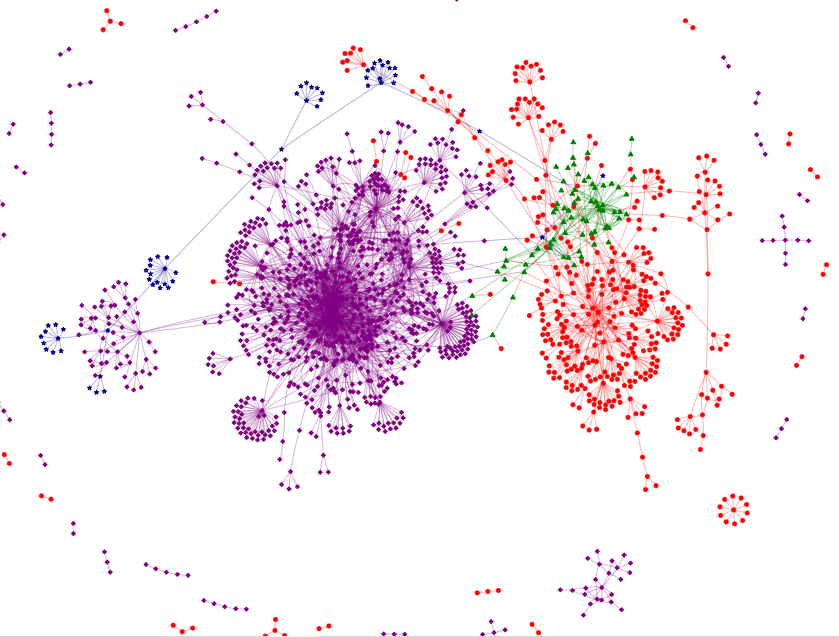
\includegraphics[scale=0.5]{graph-vis}
    \caption{Graph Data - When a user clicks on the Load Graph Network button
}
    \label{fig:graph-visualization}
\end{figure}


When visualizing the metadata entities and creating the relationship, imagine any human analyzing the graph entities. Figure 6 is unlikely to be analyzed by a single person within the organization and it will be very challenging. Therefore the need for Data Mining algorithm to extract useful information is needed. This process is covered in Linked Enterprise Data step two (see section 4.2) 


\clearpage
\maketitle
\section{Linked Enterprise Data}
To understand the topic of this dissertation it is important to understand the Linked Enterprise Data because in the dissertation Linked Enterprise Data framework is used to automate and integrate SAP Graph API with Essential Architecture API.

Linked Enterprise Data is a concept and approach that aims to seamlessly connect and integrate data from various sources within an organization. It involves establishing meaningful relationships and links between different data entities, allowing for a holistic view of the data landscape.

In Linked Enterprise Data creates a unified warehouse, and through some API, or standard formats like RDF (resource description framework) the data is shared. These data are exposed for searching, accessing, and extracting new knowledge from the systems. Linked Enterprise Data provides solutions for productivity, scalability, flexibility, continuity, and reversibility. There are three steps to create a linking process, business objects are themselves connected. Using Linked Enterprise Data, navigation becomes easier. \parencite{rao2017}

Step one is open data to create links, in our case, we have extracted the data from the SAP Graph, created the relationships between the data, and uploaded the data to the Neo4j graph database. Step two is to produce new information from the links and relationships of the data, while there are 1998 entities, producing new information is challenging, there using machine learning, and data mining techniques, the graph data were producing some useful information, which is discussed in section 4.2. The final step is to extract the data object for visualization or business intelligence purposes. In the final stage of linked enterprise data, essential architecture API is used to visualize processes and organize data management, and information layers.

\begin{figure}[ht!]
    \centering
    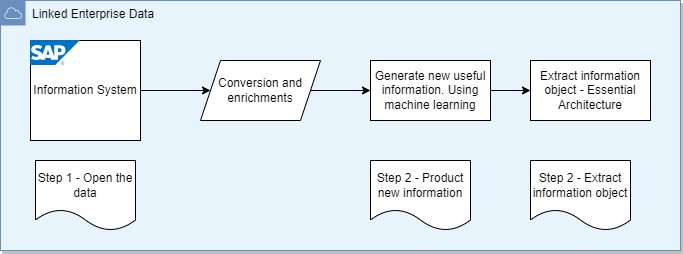
\includegraphics[scale=0.5]{linked-enterprise-data}
    \caption{Linked Enterprise Data - 
In general, the linked enterprise data has three steps, each step is required to produce useful information for the organization.
}
    \label{fig:LED}
\end{figure}

\maketitle
\subsection{Step One - Open the Data}

The first step of Linked Enterprise Data is that the data needs to be accessible within the organization through any technology such as HTTP endpoint, database, RDF, and so on. Since the data returned by the SAP Graph is in graphical representation, the decision to adopt the Neo4j graph database. Graph database management system is designed to handle, and process connected data efficiently. Unlike traditional relational databases, which store data in tables and rows. A graph consists of nodes and edges, like a graph database.

Neo4j is a graph database that organizes a graph-based model, making it an ideal choice for applications that deal with complex and interconnected data structures. The fundamental building blocks of Neo4j are nodes, relationships, and properties. Nodes represent entities in the database, such as people, products, or locations, in the case of SAP Graph, entity name, with additional information is stored as properties, while the edges are relationships connected between nodes. \parencite{miller2013}

The figure below shows the SAP Graph database like the graph shown in Figure 4, however, there is a difference between the two, firstly the graph contains more data called properties, and secondly, the data can be used to be fetched by complex read queries, and it easily to maintain, and optimize. 

In addition, the query can be performed on the properties of each node, and these properties can also be viewed as the figure below shows. 


\begin{figure}[ht!]
    \centering
    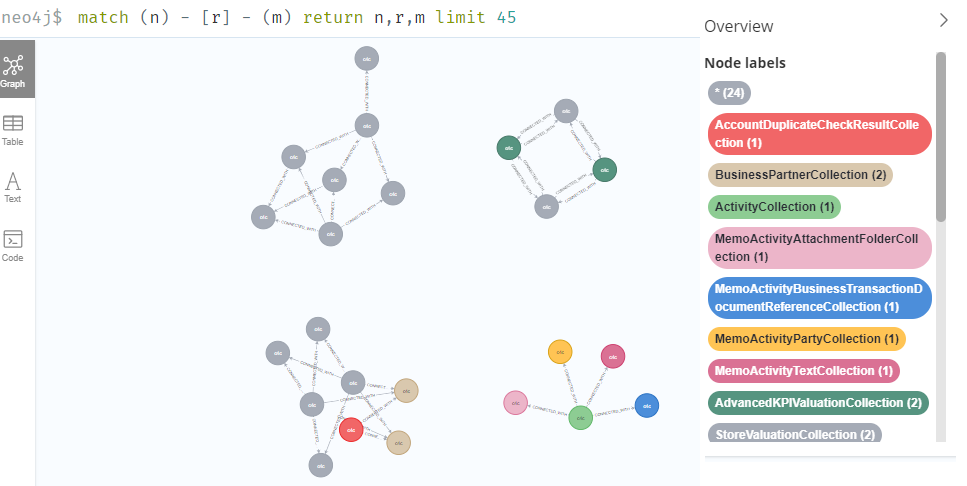
\includegraphics[scale=0.47]{neo4j-graph}
    \caption{SAP Graph Data on Neo4j - 
The graphical representation of entities with each node contains additional properties}
    \label{fig:neo4j-graph}
\end{figure}

\begin{figure}[ht!]
    \centering
    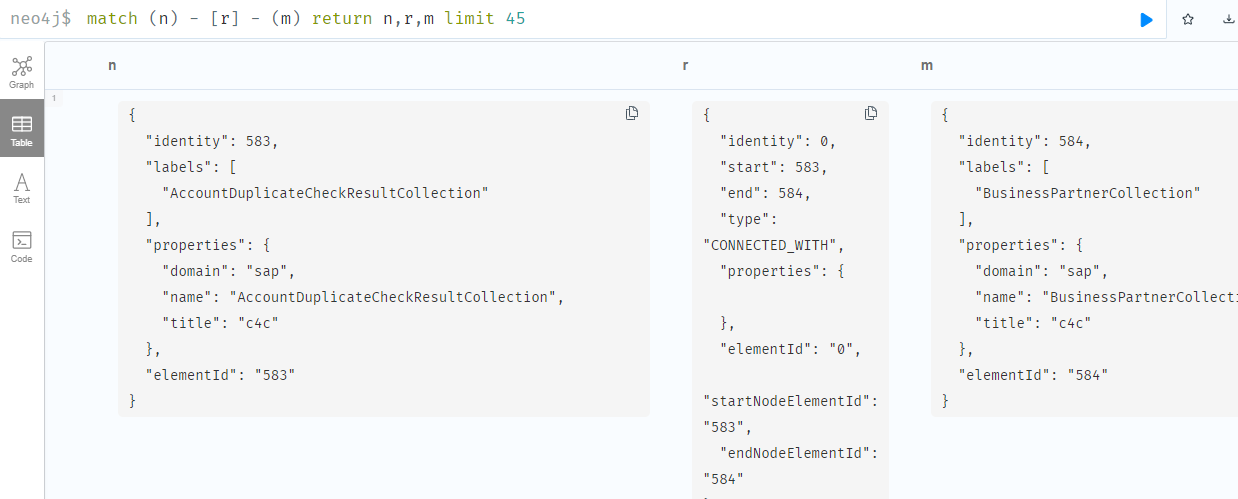
\includegraphics[scale=0.35]{neo4j-table}
    \caption{Node Properties - 
Detail of each node, each node contains properties}
    \label{fig:neo4j-table}
\end{figure}

In the context of Linked Enterprise Data, where relationships between different data entities are essential, the graph model provides a natural and intuitive way to capture and visualize these relationships. It allows for efficient traversal and querying for complex networks of data, enabling a comprehensive understanding of the data landscape. Linked Enterprise Data often involves the integration of data from diverse sources and domains \parencite{rao2017}. Neo4j’s flexibility and adaptability make it a powerful tool for handling various types of data, regardless of their structure or format. Whether it’s internal data from different departments or external data from partners and suppliers, Neo4j can seamlessly integrate and manage the interconnected data. 

Lastly, Neo4j’s integration with machine learning libraries and tools allows organizations to apply advanced analytic and data science techniques to their Linked Enterprise Data. This empowers organizations to gain deeper insight, identify patterns, and make predictive analyses based on interconnected data. Neo4j data science provides tools for data mining, and unsupervised learning such as K-means clustering, similarity scoring, and so on. \parencite{hodler2022a}

To enable the Neo4j Data Science plugins, go to the database, and select plugins. Under the plugins tabs find Graph Data Science and click Install. This will enable Data Science algorithms, which will be applied to the database. 

Now as per step one of Linked Data Enterprise, a person within the organization must be able to query the data to extract only the needed information. This can be achieved by entering the name of the required entity. The outcome result shows the entity with its relationship with the other entities.

The integration of Neo4j plays a vital role in implementing Linked Enterprise Data, facilitating efficient data management and decision-making processes. One significant advantage of Neo4j is its ability to interact with individual entities, allowing for focused analysis and a deeper understanding of the organizational structure within specific domains. Given that the SAP graph API returns a substantial number of entities (1998 entities), visualizing all of them simultaneously poses a challenge and may lead to difficulty in comprehensive analysis. However, with Neo4j's capability to handle single entities at a time, the entities can be examined more precisely and accurately.
Moreover, the use of Neo4j not only supports the implementation of Linked Enterprise Data but also opens opportunities for leveraging machine learning tools on graph data. For instance, applying K-means clustering can help identify clusters based on similarities among entities, providing valuable insights into various organizational aspects.

With the combination of Neo4j's graph database and machine learning capabilities, the research stands to gain deeper insights and more useful information from the integrated data. This enhanced level of analysis can aid in making informed decisions and discovering hidden patterns or relationships among the entities. Overall, the incorporation of Neo4j in the research's methodology contributes to the efficiency and effectiveness of data management and analysis processes, advancing the understanding of the automation and integration of SAP with Essential Architecture and Linked Enterprise Data. \parencite{hodler2022a}


\begin{figure}[ht!]
    \centering
    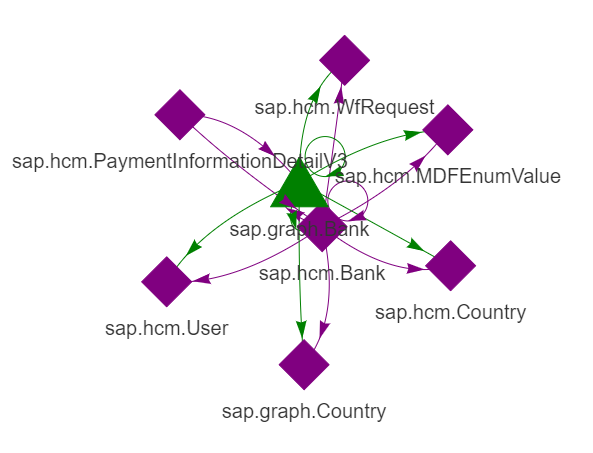
\includegraphics[scale=0.6]{graph-open-data}
    \caption{Entity Relationship - 
A single entity with a relation with the other entities}
    \label{fig:graph-open-data}
\end{figure}


\maketitle
\subsection{Step Two - Product New Information}
In the context of Linked Enterprise Data, the process of creating and interlinking data from sources often leads to the production of new information. This is one of the key benefits of adapting data principles and semantic web technologies. Since the SAP Graph produces 1998 entities, extracting and analyzing useful information is a challenge. Data mining is a technique to discover patterns or trends in data. Data mining is also a technique of identifying relationships between or extracting valuable information from the dataset. It involves producing insights and meaningful knowledge from the data. The generated outcome can be used in decision-making, optimization purposes, and predictions. Data mining is also known for knowledge extraction. \parencite{chen1996}

The data mining process consists of four basic steps. 
\begin{enumerate}
    \item Setting Objectives – Data scientists and business stakeholders work together to define a business problem.
    \item Data Preparation – Identify which set of data the algorithm will help to answer business questions. The step also involves cleansing the dataset and transforming the dataset.
    \item Application Data Mining – There have been different data mining algorithms developed, in the dissertation we have applied the Association Rule Mining technique.
    \item Evaluating Model – The results are interpreted, understanding the results, and validating the outcomes.
\end{enumerate}

Data Mining can be classified into three categories, association, classification, clustering, and predictions. The association is a rule-based technique for finding relationships between variables in large datasets, classification is a technique to identify the type of data, for example in our dataset the use of classification can use to generate which entities belong to which type of class, however, in the dissertation, we have not explored the classification data mining algorithms. Clustering in data mining is a grouping of data by the similarities, this technique can be used to group the entities on the bases of similarities by the attributes, using clustering data mining would not necessarily produce useful information for the dissertation, because the attributes in one linked entity can be different from its another linked entity. Prediction is another category of data mining named like a machine learning regression model, data mining can also be used to predict, it is unsupervised learning because the datasets are not labeled. In this dissertation, prediction is not required. \parencite{madni2017}

The reason to use data mining techniques is that in the essential architecture information and data view, the required are data objects, data object attributes, data specialization and generalization, and other information system-related information. Capturing all the 1988 number of entities to the Essential Architecture would not produce clear and proper visualization as data it is a large dataset, furthermore, linked enterprise step two requires producing new information, therefore, it is a good idea to perform machine learning algorithms on a graph data provided by SAP Graph Data.

\maketitle
\subsubsection{Using Associate Rule Mining}

Since SAP Graph data is a metadata of the entities, it contains relationships and some information to extract therefore Association Rule Mining is a good fit for this problem. Association Rule Mining is a rule-based algorithm, and it is used for finding the set of relationships between the data \parencite{kumbhare2014}. In association rule mining a simple correlation is drawn between two or more items, often of the same type to identify the patterns. For the SAP Graph Data, we identify the relationship of one entity with another. Furthermore, the metadata provided by the SAP Graph Data also contains other attributes of an entity which can also be used to get more insightful information about the data.

The association rule has two parts, an antecedent, and a consequent. The antecedent is the "if" part of an association rule or a rule-based model. In association with rule mining, it represents the itemset or a combination of items that act as a condition or premise for the occurrence of another item or set of items. An association rule expresses a relationship between different items in a dataset, stating that if the antecedent is present, then the consequent is likely to be present as well. For example, in SAP Graph entity the data {Bank} =>{Country}, this rule suggests if there is a Bank (the antecedent) entity there is a likelihood that Country (the consequent) will also be linked.

The support in the association rule mining is the frequency of occurrence of interest, in the SAP Graph data case, it is the entity. Frequent itemset represents which support is greater or equal to a minimum threshold. Consequent is the “then” part of an association rule. In association rule mining, it represents the item or set of items that are predicted to be present in the dataset when the antecedent is satisfied. Continuing with the previous example {Bank} => {Country}. The model predicts if there is an entity Bank it is more likely to have a relationship with the Country.

The association rule mining also provides the model evaluation metrics, first calculating the support $\sigma(X + Y) /$ total transactions. Where $X$ and $Y$ are sets of items or itemsets. The $\sigma$ is often used in mathematics to denote the summation or total of a set of values. Total transactions are the number of nodes or rows in a dataset. Confidence represented as $c$ is $\text{Supp}(X \cup Y) / \text{Supp}(X)$, counts how many times the itemset $Y$ appears which is also included in the union of $X$ with $Y$. Lift represented as $l$, is calculated by the rules such as $\text{Lift}(X \Rightarrow Y) = \text{Conf}(X \Rightarrow Y) / \text{Supp}(Y)$. Lift if it is greater than 1 means both sets appear together more times, while lift if less than 1 means appear fewer times \parencite{kumbhare2014}.

There are different types of algorithms for association rule mining. Apriori algorithm is association rule mining is used for the dissertation. The Apriori technique is the first association rule mining technique. It works iteratively, and the key idea behind is based on the “Apriori Property” which states that if an itemset s frequent, all of its subsets must be frequent \parencite{yuan2017}. Other are the Eclat algorithm and the FP-growth algorithm.

Association rule mining can also be used with the graph data, the association rule mining helps to discover regularities between entities and relationships. Studies show that the association rule mining pattern generates a tree-like structure. Therefore, producing new information, which can be used in Essential Architecture to capture data for data object instances, and define data generalization and data specialization. (see Section 4.4)

\maketitle
\subsubsection{Web Application and Association Rule Mining}

Navigate to the essential architecture page and click the “process with association rule mining” button. This will execute the association rule mining algorithm in the backend web application. The outcome is then mapped to the graph representation using the same library as in the sap graph’s graph representation.

\begin{figure}[ht!]
    \centering
    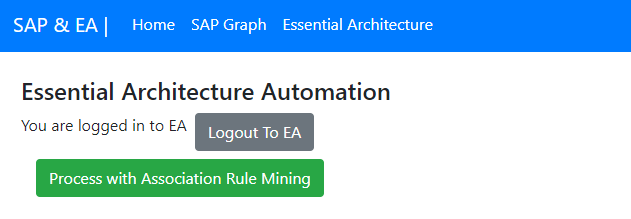
\includegraphics[scale=0.6]{ea-ar}
    \caption{AR-mining button - 
The button executes the association rule mining algorithm to produce new information.}
    \label{fig:ea-min-ar}
\end{figure}

Figure 12 is applied on the configuration of minimum support equal to 0.0009, minimum confidence equal to 0.2, minimum lift is 3, and minimum length equal to 3. The algorithm is applied to all the entities in the dataset which were fetched from the SAP Graph. The algorithm produces new and more optimized results. If we drill down to one graph, the information will be clearer and visualized. Notice in the figures below the output in the generated graph is more concise and accurate. Also, notice that using the data mining algorithm produces information that cannot and understood by the human eye. Analyzing Figure 12, we observe that the graph is associated with jobs, job specifications, applied candidates, job applications, and other related elements. Hence, it can be inferred that this graph captures entities relevant to the hiring process for a position. As mentioned earlier, this graph is generated using the minimum configuration applied to the data from SAP Graph. However, if we decrease the number of support and confidence, the association rule mining is likely to produce more graph data.

The flexibility of this approach allows us to adjust the configurations based on business and analytics requirements to obtain the desired information. Figure 13, The graph displayed below illustrates more nodes and connections because the minimum support is set to 0.0006, minimum confidence is set to 0.1, minimum lift is set to 3, and minimum left is set to 2. These parameter changes contribute to a more comprehensive representation of the relationships and entities associated with the hiring process.

\begin{figure}[ht!]
    \centering
    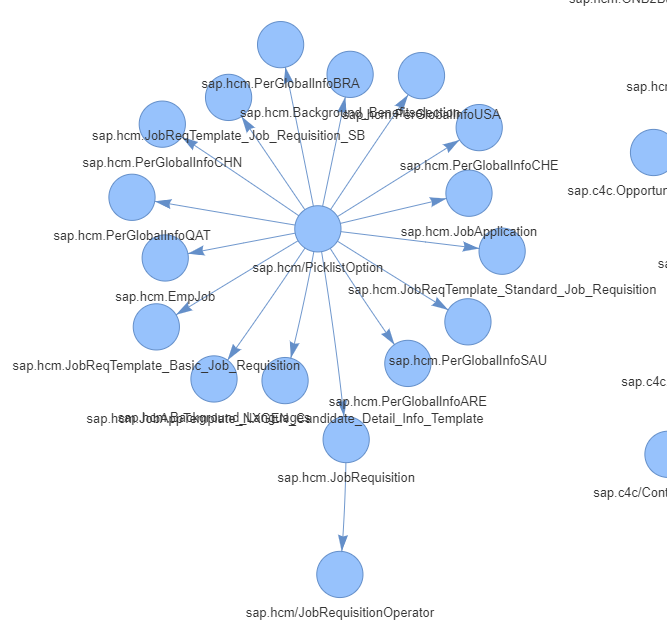
\includegraphics[scale=0.5]{ar-max-output}
    \caption{Association Rule Mining Output - 
The association rule mining overall outcome on a minimum configuration.}
    \label{fig:ea-max-ar}
\end{figure}

\begin{figure}[ht!]
    \centering
    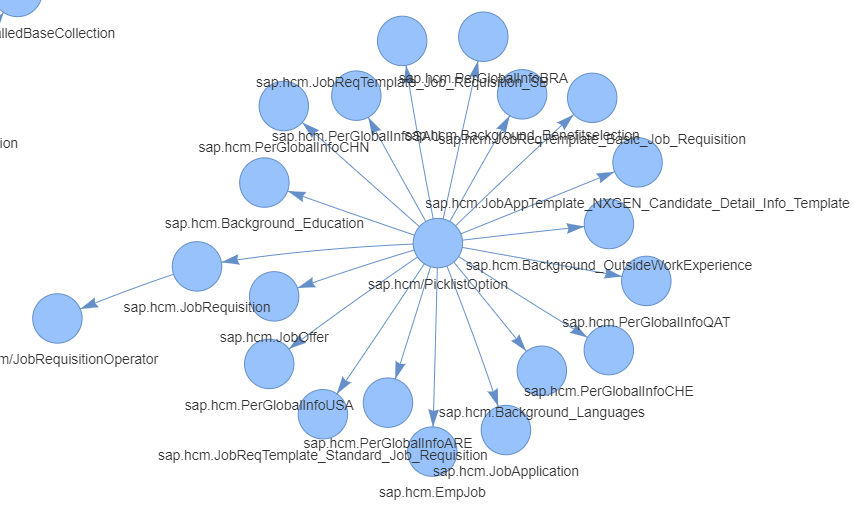
\includegraphics[scale=0.5]{ar-min-output}
    \caption{Association Rule Mining Output - 
The association rule mining overall outcome on a minimum configuration.}
    \label{fig:ea-ar}
\end{figure}

The lower the minimum support and confidence the association rule mining produces more information however it is more computationally intensive to use the lower number for support and confidence.
In summary, association rule mining is a valuable technique for extracting and generating information. According to the Linked Enterprise Data guidelines, the second step involves generating new information that is beyond human capacity to analyze and visualize. Data mining plays a crucial role in analyzing these entities and relationships. The resulting output is now automated and feeds into the Essential Architecture for further exploration.

\maketitle
\subsection{Step Three - Information Object Extraction}

Once the output is received from the data mining algorithm with the information. The output is used to extract the object for essential architecture. In the dissertation, the extraction of objects to upload and capturing of these data in the essential architecture has been automated through the REST API provided by the essential architecture.

EAS was developed and incorporated in 2000. EAS aimed to improve the professionalism, business process, and value delivered through enterprise architecture. It provides the architecture to the organization that what we do, how we can do it, and how we can use skills. 

\begin{figure}[ht!]
    \centering
    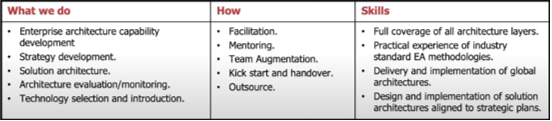
\includegraphics[scale=0.8]{ea-what-how-skills}
    \caption{EA Architecture facilities - 
EA explanation about what and how they do}
    \label{fig:ea-facilities}
\end{figure}

Enterprise Architecture (EA) is a strategic approach that aims to align an organization's business objectives and strategies with its information technology (IT) infrastructure. It provides a comprehensive framework for designing, planning, and overseeing an organization's IT systems. In doing so, it offers insights into the organization's structure, processes, components, and how they interact with technology.

The main goals of Enterprise Architecture are as follows:
\begin{enumerate}
    \item Alignment: Ensuring that IT projects and investments are in sync with the organization's business objectives and strategies.
    \item Integration: Facilitating the seamless integration and compatibility of IT systems and components across the entire organization.
    \item Standardization: Establishing guidelines, principles, and standards to promote consistency, efficiency, and the ability to reuse IT solutions.
    \item Optimization: Maximizing the value of IT resources, processes, and investments while minimizing duplication or unnecessary overlaps.
    \item Change Management: Assisting in navigating the complexities and impacts of organizational changes, such as mergers, acquisitions, or technology upgrades.
\end{enumerate}

By leveraging Enterprise Architecture practices, organizations can enhance their agility, efficiency, and decision-making capabilities. Moreover, it enables them to foster innovation and adaptability in response to the rapidly changing technology landscape.

\begin{figure}[ht!]
    \centering
    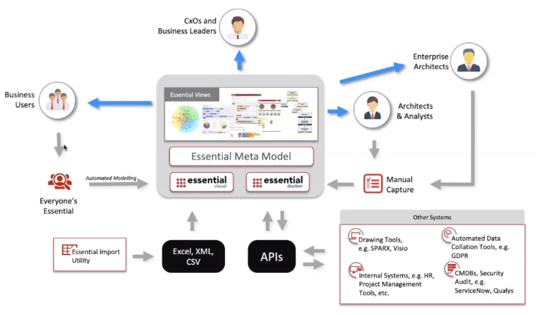
\includegraphics[scale=0.8]{ea-architecture}
    \caption{EA Architecture - 
Core Meta Data contains the layers and the three types of capturing data }
    \label{fig:ea-architecture}
\end{figure}

Metadata, short for "metadata," refers to additional information or details about a particular set of data. It acts as a descriptive prefix that provides information about the content and characteristics of the data, regardless of its format, such as videos, images, spreadsheets, databases, or web content. In simpler terms, metadata can be thought of as a summary or contextual information that aids IT industries in understanding what customers want and how to enhance their business. Regardless of the type of data, whether it is organized and structured or unstructured, the presence of metadata is crucial. It enables organizations to efficiently discover, manage, and analyze data, making it an essential aspect of modern data-driven industries. By leveraging metadata, businesses can gain valuable insights, improve their decision-making processes, and enhance their overall operations to meet customer needs effectively \parencite{marr2021}. For the dissertation, the information layer of the essential meta-model is used. However, for the dissertation, other essential meta-models were also explored.

\begin{figure}[ht!]
    \centering
    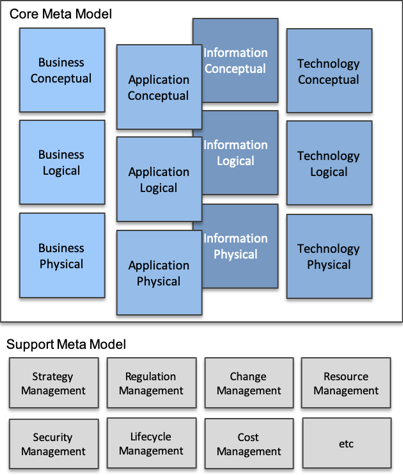
\includegraphics[scale=0.8]{ea-meata-model}
    \caption{EA MetaModel  - 
Essential Architecture contains core metamodel and supporting metamodel }
    \label{fig:ea-metamodel}
\end{figure}

\maketitle
\subsubsection{Utilizing Essential Architecture}

Like Object Orient Programming, A class can be abstract or concrete, only concrete classes have an instance in it. The classes are the layers, each layer contains nested classes, for conceptual, logical, and physical layers class. Each conceptual, logical, and physical layer contains a concrete or abstract class. The filled red circle represents the concrete class, while the other represented as abstract class.

\begin{figure}[ht!]
    \centering
    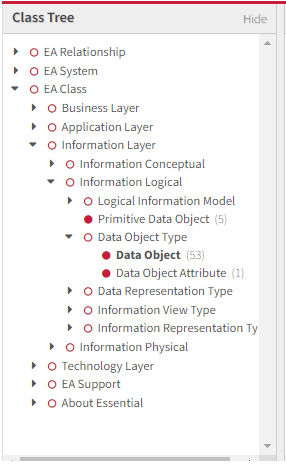
\includegraphics[scale=0.8]{ea-class}
    \caption{EA Class  - 
Classes are abstract and concrete classes }
    \label{fig:ea-class}
\end{figure}

For the SAP Graph entity data visualization and processing, business, technology, and application layer are not explored because the fetched from the SAP Graph are related to the information layer. Inside the Information layer, Data Objects, Data Object Attributes, Primitive Data Objects, Information Concepts, Data Subjects, and Information Domains are consumed. However, for the sake of understanding and benefit of Essential Architecture, in the dissertation, other classes are explored. An instance is a data representation of the class. An instance is the captured data which contains information about the different processes, security, and related data. For Instance, the Data Object class can have an instance, the instance of Data Object can have data attributes such as Name, Data Subject instance, Data Category instance, Data Attribute instance, Data Object Specialization, and Data Object Generalization class instance, and so on.

Essential Architecture Cloud has exposed the REST API endpoints to the consumer, the API is used to interact with the essential architecture Cloud, and to capture data this API comes in handy. With any programming language, the REST API can be consumed. For the dissertation to automate the Essential Architecture Cloud process, with the help of Python programming language using REST API was achieved. To connect with Essential Architecture Cloud, the consumer needs to generate the API token. Each user account has its own Tenant API key, the key can be fetched from the user profile on the top of the page, and navigate to the settings, scroll to the bottom of the page. Lastly, by using the essential architecture login API, a user needs to pass an email address and password along with the API key. The top figure shows the API key is passed inside the header, while the username and password are passed inside the body. This will return the bearer token which is valid for five minutes, and the refresh token, which is valid for 24 hours, the refresh token is used to create a new bearer token without passing the username and password over again.
The essential architecture provides instance API for creating the instance on the essential architecture cloud. The different class instance contains different types of request body which needs to handle by the integrating application. To use the automation feature for the essential architecture, navigate to the web application essential architecture page and click login. 

Once the user is logged in the application will display Logout, Create Information Concept, and Process with Association Rule Mining. The logout button deletes the stored bearer token and refreshes the token from the session. Create Information Concept is used to create information concepts, information domain, information view, and data representation inside the essential architecture. When the user clicks on the button “Process with Association Rule Mining” it will run the association rule mining algorithm, and generate information, using the generated graph data, data objects, data generalization, and data specialization are extracted. Generalization and specialization are the concepts of object-oriented, where generalization is the subclass while specialization is the superclass \parencite{sahay2016}. The extracted data first removes the existing instances in the data object class and recreates the data object instances.




\begin{figure}[ht!]
    \centering
    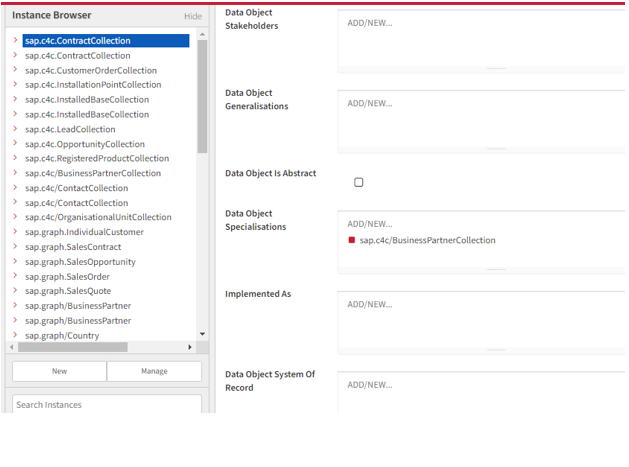
\includegraphics[scale=0.7]{ea-instance}
    \caption{EA Instance  - 
Instance created by using essential architecture API }
    \label{fig:ea-instance}
\end{figure}
\begin{figure}[ht!]
    \centering
    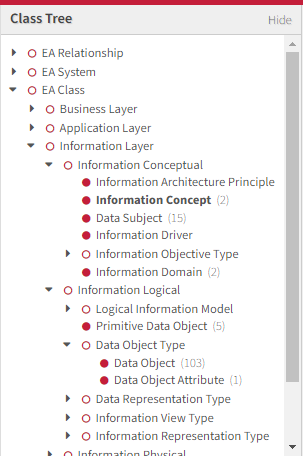
\includegraphics[scale=0.7]{ea-ic-2}
    \caption{EA Information Conceptual Layer  - 
Information conceptual layer created using REST API  }
    \label{fig:ea-information-concept}
\end{figure}
\begin{figure}[ht!]
    \centering
    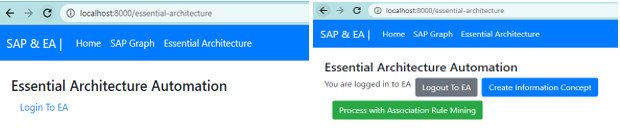
\includegraphics[scale=0.7]{ea-web-2}
    \caption{EA Using Web Application  - 
Automating EA instance creation using REST API }
    \label{fig:ea-webapp}
\end{figure}

The reason to use information concept, information domain, and data subject while using data object and data attribute, is because the information concept, information domain, and data subject. Information concepts represent high-level information, information concept helps organization in categorizing data. The information domain represents a higher-level group or category that encompasses related information concepts. It defines a boundary within which various information concepts are organized based on their similarities and relevance. Information Domains are used to provide a logical structure to the data and make it more manageable and understandable. A Data Subject is an object or entity about which data is collected, stored, or managed. It can be considered a real-world entity or an abstract concept. Data Subjects are typically represented as the main entities in a data model and are associated with attributes that describe their properties or characteristics.

\clearpage
\maketitle
\subsubsection{Essential Viewer}

The important part of the dissertation is to automate the process of data collection from SAP Graph and integrate the data with the essential architecture. The data provided by SAP Graph is huge and it is challenging for a human to analyze. Therefore the dissertation uses the provided REST API, which has been integrated and automated. Now after capturing data and publishing it to the viewer. The data can be visualized by the essential viewer.

The essential viewer is the tool provided by the essential architecture for visualizing, managing, and analyzing the organization's data. After capturing the organization's data, and it is published to the viewer, the user will be able to visualize the data. Essential Viewers comes with APR-VM visualization and data management layer. APR-VM and data management layer is advanced license.

Following are the visualizations and analyses that can be used and when they can be used.

\textbf{Enterprise} – In the Enterprise section, there are 17 different types of dashboards, including IT Asset Dashboard, Strategic Goals Models, Program Plans, Supplier Impact Map, and even NIST for cybersecurity.

\textbf{Business} – In the Business section, there are 15 different types of dashboards, each serving various purposes to visualize and analyze the business domain of an organization. This includes Business Capability Dashboards, mainly used for monitoring decisions within the organization, and Business Capability Application Fit, which provides a high-level graphical representation of how the application portfolio supports business capabilities. The Business section also contains Business Process Management Dashboards, Value Stream Summaries, and Business Domain Processes. When used together, these dashboards can benefit the organization and help understand how to optimize business processes.

\textbf{Application} – The Application section contains information about the applications within the organization, including services inside the applications, information dependency, cost, and more. The dashboards provided for this type of analysis include the Application Reference Model, Application Dependency Diagram, Application Information Dependency Diagram, and Cost Summary. There are 15 types of dashboards provided in the Application section.

\textbf{Information and Data} – The Information and Data section is used in the dissertation because the data returned by the SAP Graph is metadata of entities. The Information Reference Model provides information concepts, while the Data Subject Summary shows key relationships of conceptual data, and the Data Object Summary and Model provide logical data relationship diagrams.

\textbf{Technology} – The Technology section is related to the technology being consumed for the development of business processes. Consumed technology can also have security vulnerabilities, and therefore the essential architecture provides dashboards to analyze these vulnerabilities. The Technology Reference Model provides references and relationships between technologies. There are about 7 dashboards provided by the essential architecture.

\textbf{Support} – The Support section provides extra dashboards that help facilitate the analysis process for the organization. It contains dashboards such as All Instances by Class, Class Overview, Duplicate Dashboards – Key Class, and more.

\maketitle
\subsection{Data Exploration and Analysis}

The information domain contains multiple information concepts, information concepts contain multiple data subjects, and data subject contains data objects. The benefit of this relationship in the essential architecture is that it helps to organize, manage, and group information based on the business and information domain. The organization uses a legacy system, where the documentation is missing, this approach will group and organize different information in multiple information domains and concepts. Therefore solving the complex information system is much more organized and manageable.

\begin{figure}[ht!]
    \centering
    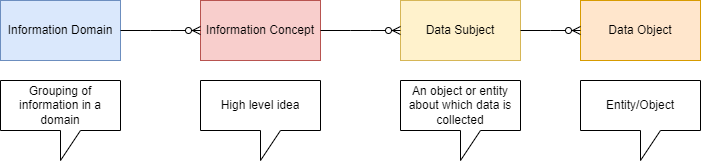
\includegraphics[scale=0.45]{ea-vis.drawio}
    \caption{EA Viewer Layers  - 
Information Domain to Data Object relationship }
    \label{fig:ea-vis}
\end{figure}

The information domain and information concept created using REST API are currently static, but it gives the basic concepts of the benefits of using the information domain and information concept. Figure 22 shows the grouping of the information domain (a higher-level) view, inside the information domain, the information concept which can be multiple inside an information domain. In the figure, the information view can also contain the data object, however, this approach does not provide organized and manageable solutions, therefore only sake of exploring the purpose the information view is created.

\begin{figure}[ht!]
    \centering
    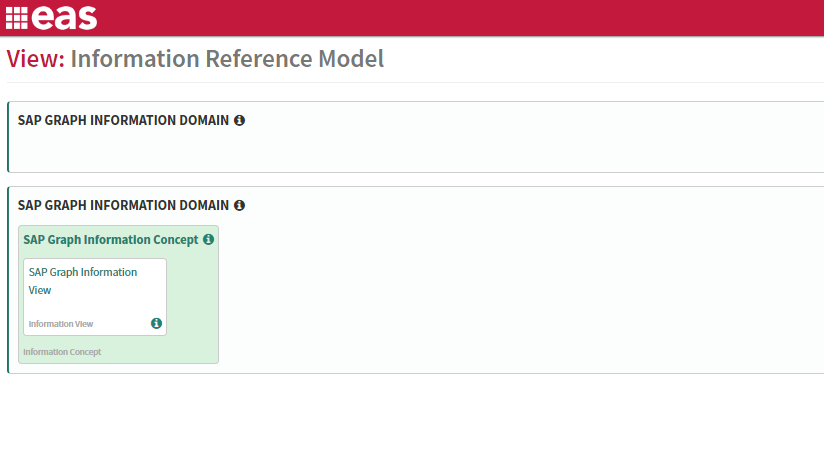
\includegraphics[scale=0.55]{information-d-andc}
    \caption{Information Domain and Information Concept  - 
A higher-level view of the information system }
    \label{fig:information-domain-and-concept}
\end{figure}

To explore deeper, then click on the information concept, the data subject can be visualized, a data subject is an object for which the data is collected and managed shown in Figure 24. Inside a data subject, the data object can be seen. This is the entity that is provided by the SAP Graph API. The grouping of this information will help an organization to understand the information system for the organization. This will help enhance, maintain, and optimize the information system for a business. 

\begin{figure}[ht!]
    \centering
    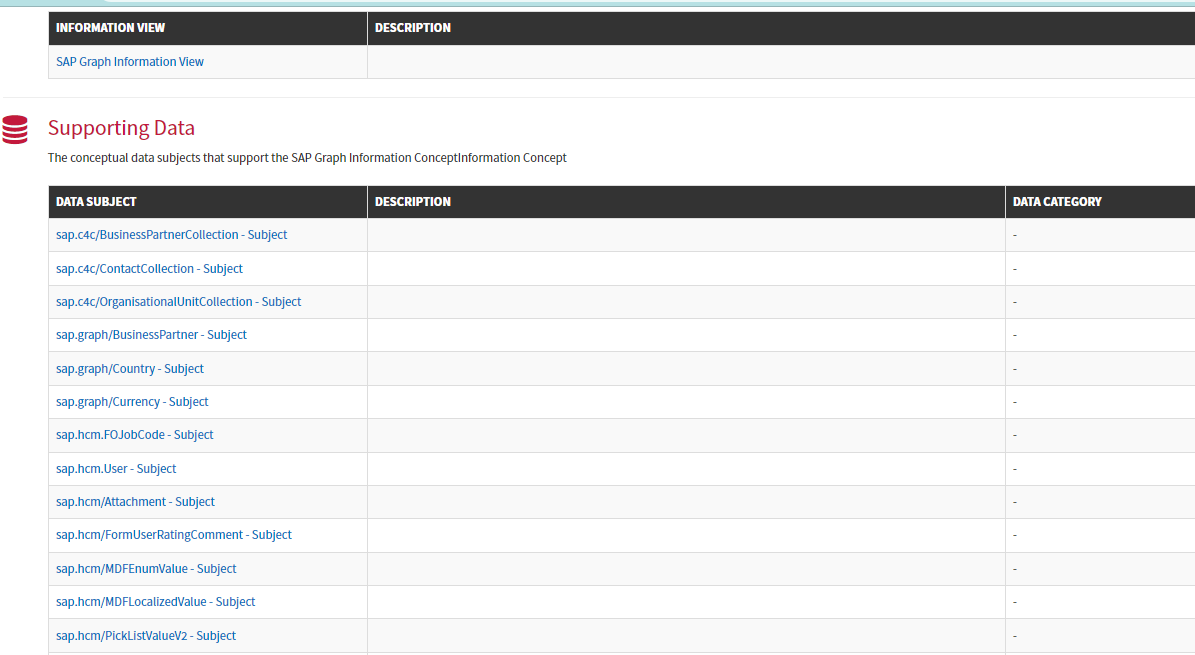
\includegraphics[scale=0.3]{ev-ds}
    \caption{Information Domain and Information Concept  - 
A higher-level view of the information system }
    \label{fig:information-concept-insight}
\end{figure}

\begin{figure}[ht!]
    \centering
    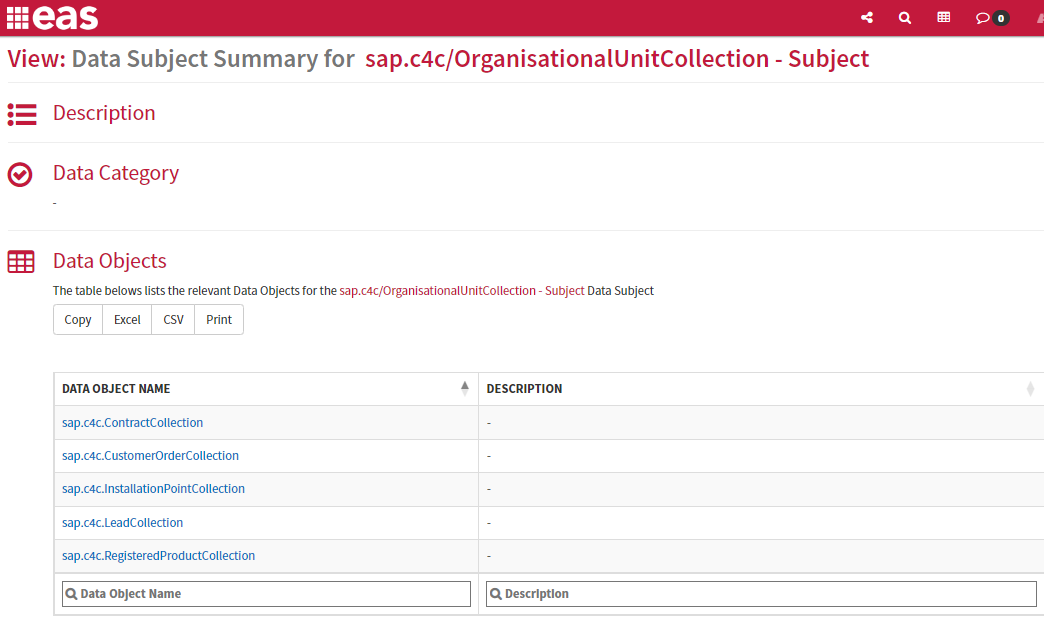
\includegraphics[scale=0.3]{ev-ds-sum}
    \caption{Data Subject  - 
Example  data subject containing data objects }
    \label{fig:data-subject-summary}
\end{figure}

In Figure 24, the data subject contains the collection of relevant data objects, these are the related entities, these entities also represent a single feature of an application or represent a focus on the simpler view of an organization information system. This helps an organization focus on a particular domain and problem to solve or optimize.

Essential Viewer tackles the challenge of analyzing data collected from SAP Graph and integrating it with the essential architecture. By utilizing the provided REST API and the essential viewer, organizations can efficiently capture, visualize, and analyze vast amounts of data. The diverse range of dashboards and analyses offered by the essential architecture caters to specific organizational needs, enabling businesses to optimize processes and make informed decisions. Through the exploration of information domains, concepts, data subjects, and data objects, the dissertation emphasizes the importance of organized information management for enhancing overall efficiency and understanding complex information systems. The benefits of using the above approach and integration of SAP Graph and essential architecture using the linked enterprise data framework and data mining algorithm are discussed in section 5.


\maketitle
\section{Case Study}
The information system within an organization often becomes a legacy, and within an organization, the documentation is missing. Businesses around the world are evolving rapidly and the need to keep up with the competitor is challenging. The dissertation offers various advantages to an organization across different dimensions. In the dissertation, the focus is the case study. In the case where SAP Graph provides the entities metadata, the entities in the given system were around 1988 entities. The challenge of integrating the SAP Graph with Essential Architecture API while producing the analytical and useful information from the process.

Using the Linked Enterprise Data framework, which is a three-step process. First, the data should be open and accessible within the organization. Using the Neo4j graph database, this step can be easily achieved. The reason to choose the NoSQL graph database is it provides not only good support for handling and querying complex graph structures but also provides Data Science, which can be used to extract further information from the SAP Graph Data.

The Linked Enterprise Data framework needs to produce new information from the open data. This is useful for organizations to enhance, manage, and optimize the information system. Because the data is huge and so much clutter. The analysis and visualization are very challenging. Therefore for the dissertation data mining algorithm is used. The association rule mining algorithm helps identify the hidden pattern and generate useful information. The generated output of the data mining algorithm was passed into the essential architecture. Essential architecture provides API to capture the data. Since the data is relevant to the information system, entities, and data management, So using the information conceptual and logical layers to analyze the SAP Graph entity. When automating the process, there were 74 entities extracted (ignoring duplicate data objects). The reason for a lower number of entities is fetched because of current computer system memory and CPU constraints. The lower the number of confidence and support the more CPU and memory utilization and time complexity increase.

After analyzing the result, the dissertation can be able to group these entities into the following result. The data subject is the number of graphs or groups of entities fetched output from the data mining algorithm. These results are helpful for an organization to understand its information system.

\begin{table}[ht!]
\centering
\begin{adjustbox}{width=\columnwidth,center}
\begin{tabular}{|c|l|ll|}
\hline
\textbf{No.} & \textbf{Data Subject} & \textbf{No of Data Objects} & \\
\hline
1 & sap.c4c/BusinessPartnerCollection & 3 & \\
2 & sap.c4c/ContactCollection & 1 & \\
3 & sap.c4c/OrganisationalUnitCollection & 5 & \\
4 & sap.graph/BusinessPartner & 1 & \\
5 & sap.graph/Country & 1 & \\
6 & sap.graph/Currency & 3 & \\
7 & sap.hcm.FOJobCode & 1 & \\
8 & sap.hcm.User & 3 & \\
9 & sap.hcm/Attachment & 2 & \\
10 & sap.hcm/FormUserRatingComment & 1 & \\
11 & sap.hcm/MDFEnumValue & 16 & \\
12 & sap.hcm/MDFLocalizedValue & 5 & \\
13 & sap.hcm/PicklistOption & 19 & \\
14 & sap.hcm/PickListValueV2 & 2 & \\
15 & sap.hcm/User & 11 & \\
\hline
\end{tabular}
\end{adjustbox}
\caption{The Data subject with the number of data objects}
\end{table}

Table 1 shows the outcome of the data subject, which is analyzed by the organization. This gives the organization the basic structure and a clearer view of the information system. Using automation the information produced is more accurate and no redundancy is found. The mentioned entities above are 74 in the data object, inside the data subject number of the data objects is also 74. 

\maketitle
\subsection{Benefit of Automation and Integration}

In the realm of computer science, the demand for automation has experienced swift and significant growth. This surge is primarily attributed to the concept of continuous integration and delivery, wherein systems operate programmatically to minimize or eradicate manual processes. This acceleration empowers organizations to make prompt decisions and maintain up-to-date operations \parencite{wilcox2015}. 

The benefits of integration and automating the SAP Graph data and essential architecture are as follows

\begin{enumerate}
    \item The manual retrieval of SAP Graph Data has been entirely streamlined. Employees are no longer required to download data by accessing the SAP portal and subsequently analyzing it. Through seamless integration with the SAP Graph API, data remains consistently up-to-date.
    
    \item The incorporation of foundational architectural APIs for data capture eliminates the need for labor-intensive manual data entry into designated Microsoft Excel spreadsheets. This integration concurrently addresses concerns related to erroneous inputs and the accumulation of superfluous data. As an organization scales, this methodology ensures that personnel are relieved from the demands of data processing.
    
    \item Employing machine learning data mining algorithms empowers the organization to derive novel insights. This capability enables the discovery of latent patterns within the data furnished by the SAP Graph.
    
    \item The implementation of automation and integration further facilitates the organization in storing processed data within a distinct database. This repository serves as a resource for subsequent processing and in-depth analysis.
\end{enumerate}

\maketitle
\subsection{Advantages of the Linked Enterprise Data Framework}

The utilization of the linked enterprise data framework follows a structured three-step process that enhances data accessibility and utilization within an organization.

\begin{enumerate}
    \item Data is made seamlessly accessible within the organizational framework by leveraging Neo4j. This approach allows for the targeted extraction of essential data from the organizational system. Furthermore, this consolidated database serves as a foundation for the development of supplementary information systems while maintaining compatibility for subsequent operational tasks.
    
    \item The linked enterprise data framework contributes to the creation of new insights. Offering a comprehensive view of the organization's information system, it enables the organization to gain deeper comprehension and insight.
    
    \item The extraction of these derived insights for extensive analysis enhances the organization's decision-making capabilities. This capability enables the identification of potential issues and the provision of optimized solutions for the organization's clients.
\end{enumerate}

\subsection{Complexity Analysis of Automation and Integration}

The need to develop an application for automating and integration contains complexities such as technical or development complexities, hardware, and deployment complexities.

\textbf{Technical Complexity} - The development of an application centered on SAP Graph and its essential architecture API necessitates the meticulous implementation of a comprehensive software development lifecycle and process, entailing the navigation of inherent intricacies. These intricacies extend to encompass a profound understanding of the data structure provided by SAP Graph and the adept utilization of the pivotal architecture API.

In the realm of application development, testing assumes a pivotal role in ensuring the robustness and reliability of the software. Within the domain of software engineering, developers are equipped to construct unit tests and incorporate integration testing within the software program. However, the realm of complexity escalates notably when engaging in user acceptance testing. During this critical phase, stakeholders immerse themselves in real-world scenarios, meticulously scrutinizing the system's responsiveness in generating accurate and requisite outcomes.

Moreover, the sphere of technical complexity encompasses multifaceted monitoring intricacies, notably spanning logging mechanisms and performance monitoring protocols. The meticulous oversight of these dimensions ensures not only the functionality but also the optimal performance of the developed application.

In the final stretch, the integration of SAP Graph and the essential architecture further introduces complexity, particularly concerning the hardware requisites. The strategic determination of the minimal hardware prerequisites for the deployment of the software system becomes a pivotal consideration in achieving seamless integration and automation of SAP Graph and the essential architecture.

In essence, the development journey encompasses multifarious dimensions of complexity, from testing to technical oversight to hardware considerations, all converging towards the overarching goal of impeccably integrating SAP Graph and its essential architecture within a robust and high-performing application ecosystem.

Currently following Table 2 is the system specification on which the integration and automation software is developed.


\begin{table}[ht!]
\centering
\begin{adjustbox}{width=\columnwidth,center}
\begin{tabular}{|c|c|}
\hline
\textbf{Name} & \textbf{Specification} \\
\hline
Memory & 8 GB \\
\hline
Processor & Intel Core(TM) i7-8565U CPU @ 1.80GHz \\ 
\hline
OS & Windows 10 Home Edition 64-bit \\
\hline
Disk Type & Samsung SSD 870 QVO 1TB \\
\hline
Programming Language & Python 3.1 \\
\hline
\end{tabular}
\end{adjustbox}
\caption{System Specification}
\end{table}

\textbf{Time Complexities} - The execution of the automation process contains time complexities. The fetched data from the SAP Graph is about 1988 entities, the software made a 1988 HTTP request to fetch the data. The time complexity for fetching the data from the SAP Graph server depends on the downstream as well as upstream bandwidth. 

The Apriori algorithm has a time complexity that is exponential in the worst case, but it often performs much better in practice due to various optimizations. The first step of the Apriori algorithm involves generating frequent item sets of different lengths. The time complexity of this step is \begin{equation}O(k \cdot 2^{N})\end{equation}, where N is the number of items in the dataset and k is the average length of frequent itemsets. Generating candidate itemsets: The algorithm generates candidate itemsets for the next. Pruning candidate itemsets: In this step, the algorithm prunes candidate itemsets that are not frequent. The time complexity depends on the efficiency of the pruning process but is generally lower than in the previous steps. \parencite{xie2008}

The function used inside the web application has a time complexity of \begin{equation}
    T = O(n) + O(m)
\end{equation}. The pseudocode for the algorithm for creating the relationship between the entities is as follows. The function contains two main loops, one that iterates through each property in the properties dictionary and another that processes potential references within each property. Inside the function, another function contains another for loops, iterating, and finding ref properties. 

\clearpage
\maketitle
\section{Future Work}

In the future, emphasis will be placed on leveraging advanced data mining techniques, harnessing sophisticated machine learning algorithms to yield more nuanced and productive outcomes. The utilization of application realization portfolios and data management offered by essential architectures holds the potential to deliver enhanced benefits to organizations. For the dissertation, an information meta-model is used, however, in the future, the essential architecture provided APR-VM and data management viewer, using these viewers has more benefits for an organization.

\subsection{Conclusion}

In summary, the dissertation provides a sample application showing how to integrate the SAP Graph API and Essential Architecture API to integrate and by using a machine learning algorithm to fetch the new information and relevant information to automate. The reason to use data mining association rule mining is that there are 1998 entities, and uploading the extracted data to the essential architecture does not provide a clear understanding of the data. Therefore by using data mining, data can be conceptually and logically grouped. Linked enterprise data framework provides the structure processes of dealing with the information system. The use of a linked enterprise data framework helps an organization define a proper way to process an information system by opening data, producing new information, and extracting information for analysis, further processing, optimization, and so on. \parencite{galkin2016}

In the dissertation, the information concept, information domain, and data subject are a conceptual layer, with the data mining results, the data subject creates subjects for an organization, and inside the data subject the logical layer data object is attached, the data object is the nodes or entity which SAP graph has provided. Using the approach benefits the organization and users to group the set of relevant information into respective subjects and domains. By doing so an organization has a clear picture of their information systems.

\newpage
\printbibliography

\newpage
\appendix

\section{Appendix A: Ethics Form}

The ethics form

\section{Appendix B: Saunders Research Onion}
Figure 1, the consent to use the Saunders' research onion figure has been taken from the grad coach. The below figure is the screenshot of the consent.

\begin{figure}[ht!]
    \centering
    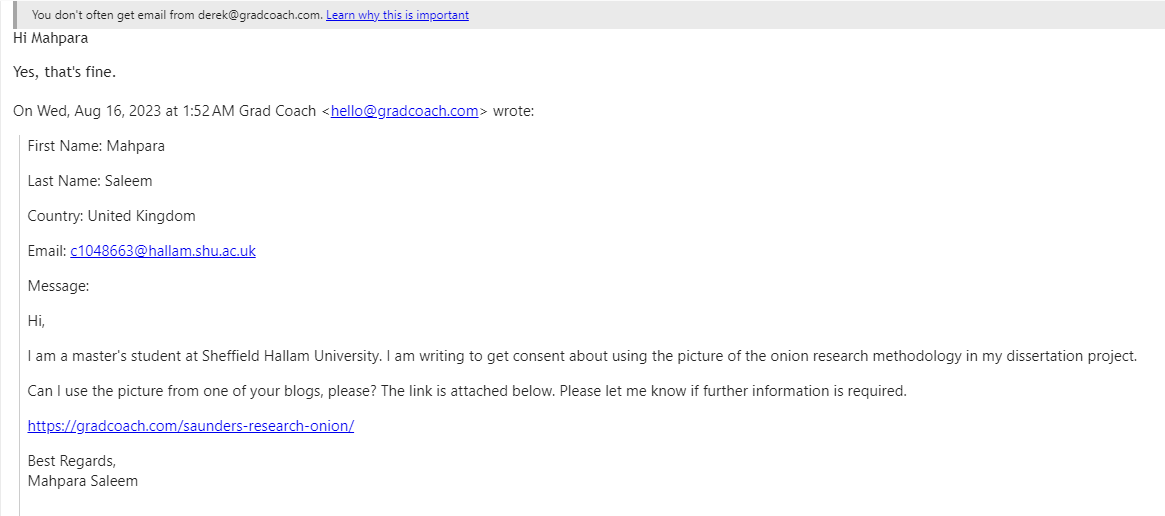
\includegraphics[scale=0.3]{onion-ring-consent}
    \caption{Consent Evidence  - 
An onion research methodology consent }
    \label{fig:onion-research-consent}
\end{figure}

\section{Appendix B: SAP Graph Data Gathering}
The SAP Graph API provides two APIs one for logging in API. This process is called OAuth 2.0. The API depends on the client id, client secrets, and redirect URI. This redirect URI is the client's application. Once the client id and client secrets are verified, the client is provided with a one-time code, which is passed to the SAP, SAP after authenticating the provided code, opens its webpage for the user to enter the username and password, once the user enters the validate credentials user is returned with an access token for accessing the resources in the SAP. The access token is JWT based and it contains the information about the authority of resources to access by users. 

To access the resource (SAP Graph) entities data, There are two APIs consumed. The first API call retrieves catalog data for the entities, this API does not contain entity data but URL path information about the retrieval of the entities' data. Using the for loop on the API, the request is made to the path provided by the SAP API to fetch all the entity's metadata. Inside the metadata, the \$ref property contains the entity name to which it is connected. 

\section{Appendix C: Essential Architecture APIs}
For integrating with the essential architecture for the dissertation the CRUD operation API was provided by the essential architecture. First using the login API to get the bearer token. The API depends on API Key which can be retrieved from the user profile under the essential architecture web application. Using the /instances POST requests to create the entities, the /instances POST request requires the class name, name to create a basic instance for the concrete class. The dissertation also deletes the existing instances to sync with the most updated data, therefore using /classes/<classname>/instances DELETE requests to delete the existing entities.

\end{document}
